\documentclass[final]{beamer}

\input{style.tex}

\usepackage[english]{babel}
\usepackage[utf8]{inputenc}
\usepackage{amsmath,amsthm,amssymb,latexsym}
\usepackage{multirow}
\usepackage[orientation=portrait,size=a0,scale=1.15]{beamerposter}

\usebackgroundtemplate%
{
    \includegraphics[width=\paperwidth,height=0.5\paperheight]{figures/TU_building.pdf}
}

\title{Towards Driving Quantum Systems in Cryogenic Environments\hspace*{1cm} \\ with the Near-Field of Modulated Electron Beams}
\author{\underline{T. Spielauer$^{1}$}, M. Kolb$^{1}$, T. Weigner$^{1}$, J. Toyfl$^{1}$, G. Boero$^{2}$, P. Haslinger$^{1}$ }
\def\correspondingAuthorEmail{thomas.spielauer@tuwien.ac.at}
\def\website{}
\institute[]{
  {\small
  $^{1}$VCQ, Technische Universität Wien, Atominstitut, Stadionallee 2, 1020 Vienna, Austria; $^{2}$EPFL, BM 3110 Station 17, CH-1015 Lausanne, Switzerland
  }
}


\begin{document}
\begin{frame}[fragile]{}
  \pgfsetfillopacity{0.80}
  \begin{block}{\Large Abstract}
    Coherent electro-magnetic control of quantum systems is usually done by
    electro-magnetic radiation - which limits addressing single selected
    quantum systems, especially in the microwave range. In our proof of concept
    experiment we want to couple for the first time the non-radiative electro-magnetic
    near-field of a spatially modulated electron beam to a quantum system in
    a coherent[1].  As the quantum system we
    use the unpaired electron spins of a free radical organic sample (Koelsch radical
    - $\alpha,\gamma$-Bisdiphenylene-$\beta$-phenylallyl) that is excited via the
    near-field of the modulated electron beam. The readout of the spin excitation
    resembles a standard continuous wave electron spin resonance experiment and is
    done inductively via a microcoil using a lock-in amplifier.

    In the long term this experiment should demonstrate the feasability of
    coherent driving and probing of quantum systems far below the diffraction
    limit of electro-magnetic radiation by exploiting the high spatial resolution of an
    electron beam.
  \end{block}
  \begin{columns}[T]
    \begin{column}{.49\linewidth}
      \begin{block}{\Large The Quantum Klystron}
        % We call our experiment the \textit{Quantum Klystron}, referencing an established
        % technology, the Klystron.

        \begin{columns}
          \begin{column}{0.4\columnwidth}
              \includegraphics[width=\columnwidth]{figures/klystron.pdf}
          \end{column}
          \begin{column}{0.6\columnwidth}\begin{center}
              {\large \textbf{Klystron}}
            \end{center}

            \begin{itemize}
              \item Linear beam vacuum tube invented in 1935, used as RF and microwave amplifier
              \item Electron beam velocity modulated by microwaves in a (buncher) cavity
              \item Velocity modulation causes current modulation
              \item Outcoupling via a catcher cavity
            \end{itemize}
          \end{column}
        \end{columns}
        \begin{columns}
          \begin{column}{0.4\columnwidth}
            % \includegraphics[width=\columnwidth]{figures/zeeman.pdf}
            \includegraphics[width=\columnwidth]{figures/qklystron.pdf}
          \end{column}
          \begin{column}{0.6\columnwidth}
            \begin{center}
              {\large \textbf{Quantum Klystron}}
            \end{center}

            \begin{itemize}
              \item Replace catcher cavity by a 2 level quantum system (QS)
              \item Drive the QS using the \textit{non-radiative electro-magnetic near-field}
                    of the electron beam.
              \begin{itemize}
                \item Either modulate in
                \begin{itemize}
                    \item \textit{time domain} - bunching / density modulation
                    \item \textit{spatial domain} - deflection
                \end{itemize}
              \end{itemize}
              \item Paint arbitrary potentials (dipole, quadrupole or multipole transitions)
              \item High spatial resolution % (electron: $\lambda_{DB}= 27.3 pm$, 202 MHz EM wave: $\lambda=1.48m$)
            \end{itemize}
          \end{column}
        \end{columns}
      \end{block}

      \begin{block}{\Large Electron spin resonance with modulated electron beams}
        The experiment resembles an electron spin resonance experiment. In contrast to
        standard electron spin resonance setups where systems are excited using microwaves,
        we use the \textit{non-radiative electro-magnetic near-field} of an modulated electron beam.

        \begin{columns}
          \begin{column}{0.3\columnwidth}
            \includegraphics[width=0.67\columnwidth]{figures/bdpa.png}
          \end{column}
          \begin{column}{0.3\columnwidth}
            \includegraphics[width=\columnwidth]{figures/zeeman.pdf}
          \end{column}
          \begin{column}{0.4\columnwidth}
            \includegraphics[width=\columnwidth]{figures/esrsetuppcb.jpg}
          \end{column}
        \end{columns}

        \begin{columns}
          \begin{column}{0.6\columnwidth}
            \begin{itemize}
              \item Sample: $C_{33}H_{21}$
                Koelsch radical ($\alpha,\gamma$-Bisdiphenylene-$\beta$-phenylallyl - BDPA)
              \item high spin density (1 free spin per 51 atoms)
              \item Proof of concept experiment at room temperature (300K) and liquid nitrogen (77K)
              % \item Excitation with microwave works at room temperature
              \item Background subtraction by differential measurement
            \end{itemize}
          \end{column}
          \begin{column}{0.4\columnwidth}
            \includegraphics[width=\columnwidth]{figures/eprsignal.png}
          \end{column}
        \end{columns}
      \end{block}

      \begin{block}{\Large Temperature dependence}
        %We want to move to a cryogenic environment. This is done due to the small signal generated by the modulated electron beam.
        %
        The thermal population ratio of spin states depends on temperature:
        
        {\large
        $$\frac{n_2}{n_1} = e^{-\frac{\Delta E}{k_B T}} = \left(e^{- \frac{\Delta E}{k_B}}\right)^\frac{1}{T}$$
        }

        \vskip1ex
        \begin{columns}
          \begin{column}{0.6\columnwidth}
            \includegraphics[width=\columnwidth]{figures/tempn2n1.pdf}
          \end{column}
          \begin{column}{0.4\columnwidth}
            \begin{itemize}
              \item $300K$ (room temperature): \\ expected $22.9 nV$ signal, $185.83 \sqrt{Hz}^{-1}$ SNR
              \item $77K$ (liquid nitrogen): \\ expected $89 nV$ signal, $1221.46 \sqrt{Hz}^{-1}$ SNR \\ expected gain $\approx 4$, SNR gain $\approx 7.7$ \\ simple to realize, our choice
              \item $4K$ (liquid helium): \\ expected $1700 nVV$ signal, $103163.45 \sqrt{Hz}^{-1}$ SNR \\ expected gain $\approx 75$, \\ SNR gain $\approx 649.5$
            \end{itemize}
          \end{column}
        \end{columns}
        \vskip1ex

        % Either remove or simpler (only for Poissonian noise)
        Averaging increases the effective SNR by $\sqrt{N}$ for $N$ iterations. \textit{Doubling SNR}
        of a single run decreases the number of required averages by a factor of four. A gain
        of 4 decreases measurement time by a factor of 16, a gain of 650 would decrease
        measurement time by about half a million.

        \begin{columns}
          \begin{column}{0.65\columnwidth}
            \begin{itemize}
              \item Initial tests by cooling BDPA sample in liquid nitrogen bath
              \item Scanned $B_0$ field, excited with microwaves (no electron beam)
              \item Compared amplitudes at 300K and 77K
              \item Resonance frequency of match drifts
              \item SIgnal gain $\approx 4$
            \end{itemize}
          \end{column}
          \begin{column}{0.35\columnwidth}
            \includegraphics[width=\columnwidth]{figures/signals300_77.pdf}
          \end{column}
        \end{columns}
      \end{block}

%%      \begin{block}{\Large Contact}
%%          Thomas Spielauer \\ 
%%          Technische Universität Wien, Atominstitut \\ 
%%          thomas.spielauer@tuwien.ac.at
%%      \end{block}
    \end{column}

    % -------------------------------------------------------------

    \begin{column}{.49\linewidth}
      \begin{block}{\Large Experimental setup}
        \begin{columns}
          \begin{column}{0.4\columnwidth}
            \includegraphics[width=\columnwidth]{figures/cryoquak02.png}
          \end{column}
          \begin{column}{0.6\columnwidth}
              \begin{itemize}
                \item Barium-Strontium cathode, electrostatic beam deflection. Current $\geq 10 \mu A$ at
                    up to $2.2 kV$.
                \item Modulation frequency $\approx 250 MHz$
                \item Two cameras imaging phosphor screens
                \item Cooling with liquid nitrogen
                \item $\leq 10^{-8}$ mbar
              \end{itemize}
          \end{column}
        \end{columns}
      \end{block}

      \begin{block}{\Large Readout and radio frequency setup}
        \begin{columns}
          \begin{column}{0.6\columnwidth}
            \begin{itemize}
              \item Inductive readout by a microcoil on a printed circuit
                board (also including impedance match)
              % \item Printed circuit board with two coils and impedance match
              \item Second microcoil for reference measurements
              \item BDPA inside microcoil (2 windings, $2.58$ x $1.14mm$
                    outer diameter, $1.5$ x $0.5mm$ sample area) in milled pocket
            \end{itemize}
          \end{column}
          \begin{column}{0.4\columnwidth}
            %\includegraphics[width=\columnwidth, angle=180]{figures/pcb01.jpg}

            %\includegraphics[width=\columnwidth]{figures/pcb02.jpg}
            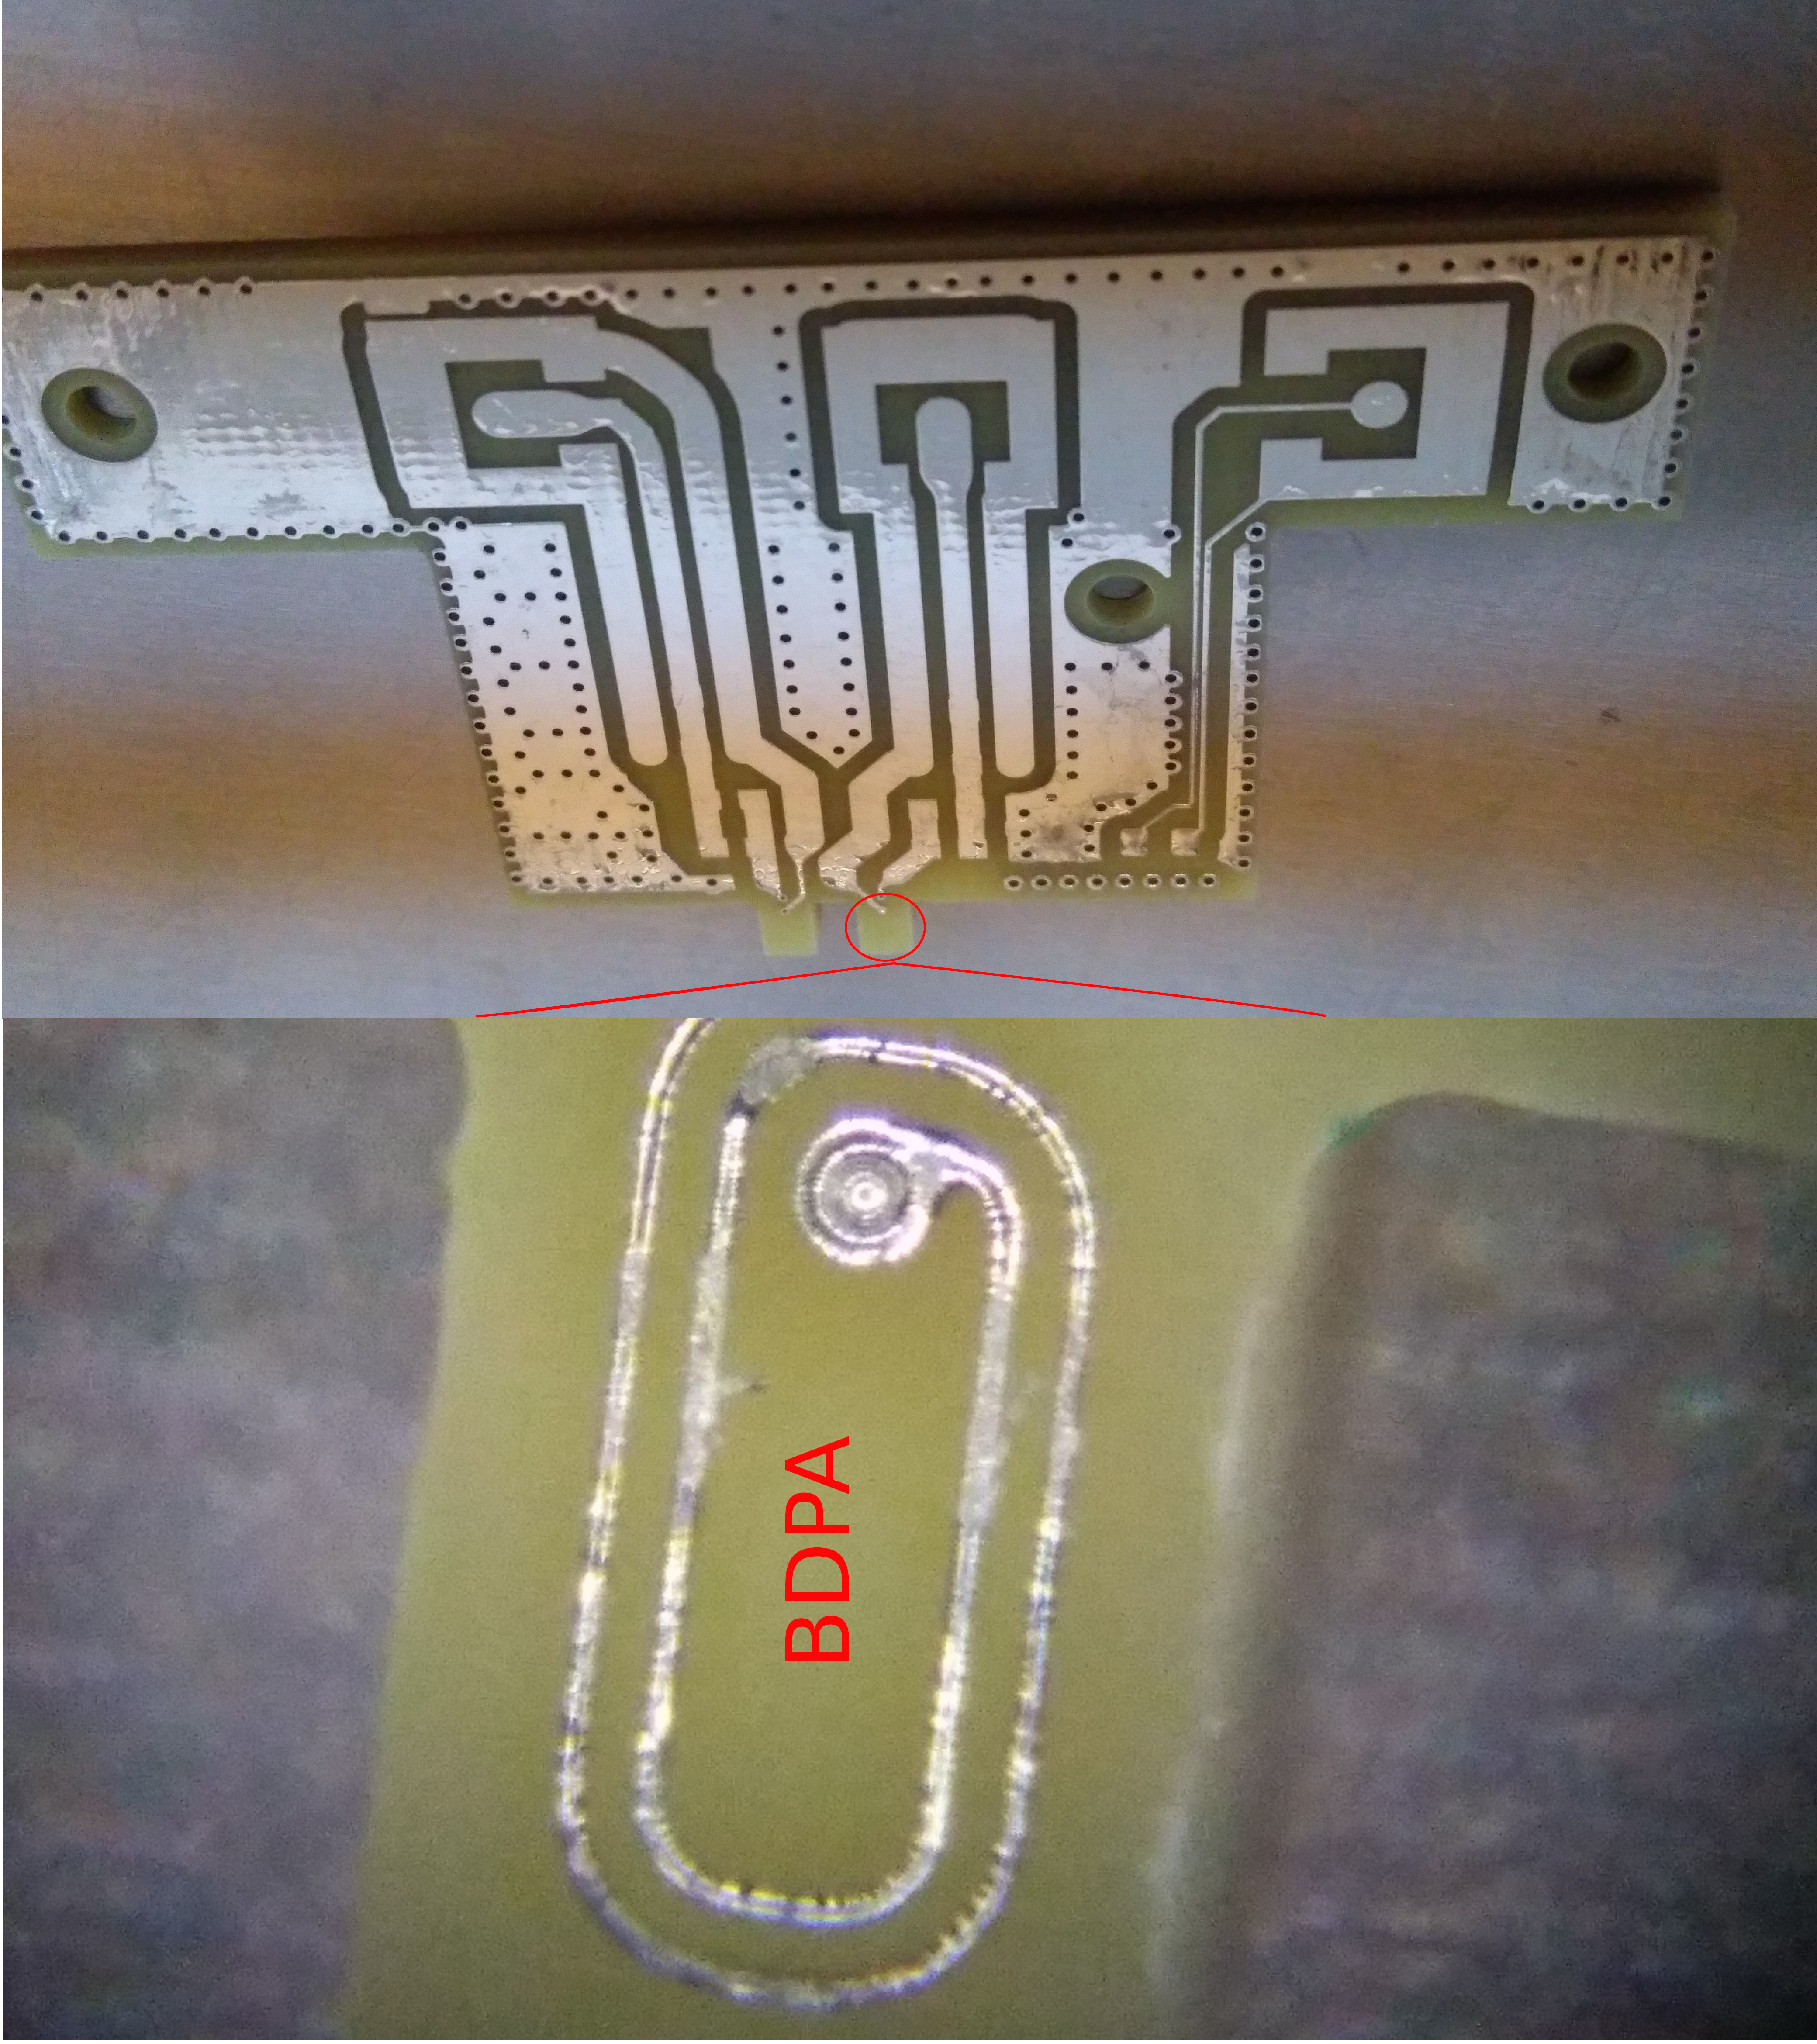
\includegraphics[width=\columnwidth]{figures/microcoilpcb.png}
          \end{column}
        \end{columns}

        \begin{columns}
          \begin{column}{0.6\columnwidth}
            \includegraphics[width=\columnwidth]{figures/rfsetup.png}
          \end{column}
          \begin{column}{0.4\columnwidth}
            \begin{itemize}
              \item Two independent channels of an AD9959 based DDS
              \item Applying $5.123 kHz$ modulation field $B_m$ parallel to $B_0$
                for lock-in detection
            \end{itemize}
          \end{column}
        \end{columns}
      \end{block}
  
      \begin{block}{\Large First runs on our room temperature setup}
        \begin{columns}
          \begin{column}{0.4\columnwidth}
            \begin{itemize}
                \item Beam at $2.2 kV$
                \item deflected at $202 MHz$
                \item Scanning distance to microcoil (\textit{slow position})
                \item Deflecting on orthogonal axis
                \item Beam wiggled by $B_m$ field
                \item Coupling of beam into microcoil
            \end{itemize}
          \end{column}
          \begin{column}{0.6\columnwidth}
            \includegraphics[width=\columnwidth]{figures/beamcoupling.png}
          \end{column}
        \end{columns}
      \end{block}

%      \begin{block}{\Large First runs on conventional test setup}
%        We did some initial tests on our setup by simply cooling a PCB containing our
%        BDPA sample in a liquid nitrogen bath.
%
%        \begin{columns}
%          \begin{column}{0.4\columnwidth}
%            \begin{itemize}
%              \item Excited using microwaves via directional coupler
%              \item Scanned $B_0$ field
%              \item Compared amplitudes at room temperature and $77K$
%              \item Resonance frequency of match
%              \item Signal gain $\approx 4$
%            \end{itemize}
%          \end{column}
%          \begin{column}{0.6\columnwidth}
%            % \includegraphics[width=\columnwidth]{figures/cryoamplitudes.pdf}
%            \includegraphics[width=\columnwidth]{figures/signals300_77.pdf}
%          \end{column}
%        \end{columns}
%
%        We saw the expected increase in signal amplitude as well as a shift of our
%        impedance match that we have to compensate for.
%      \end{block}

      \begin{block}{\Large References \& Acknowledgements}
        [1] D. Rätzel, D. Hartley, O. Schwartz, P. Haslinger, A Quantum
        Klystron - Controlling Quantum Systems with Modulated Electron Beams.
        \textit{Phys. Rev. Research 3, 023247 (2021)}
      \end{block}

      \begin{block}{}
        \begin{columns}
          \begin{column}{0.3\columnwidth}
            \includegraphics[width=\columnwidth]{figures/logo-fwf.png}
          \end{column}
          \begin{column}{0.2\columnwidth}
            \includegraphics[width=\columnwidth]{figures/logo-ffg.png}
          \end{column}
          \begin{column}{0.4\columnwidth}
            \includegraphics[width=\columnwidth]{figures/logo-oeaw.png}
          \end{column}
          \begin{column}{0.07\columnwidth}
            \includegraphics[width=\columnwidth]{figures/logo-start.png}

            START Prize 2018
          \end{column}
        \end{columns}
      \end{block}


      \begin{block}{\Large Join our team!}
        We have open positions for Master, PhD and PostDoc!

        Visit us at \texttt{http://www.haslingerlab.com/}

        E-Mail: \texttt{philipp.haslinger@tuwien.ac.at}
      \end{block}
    \end{column}

  \end{columns}

\end{frame}
\end{document}
